% xetex compatible variant that support TTF fonts according to company rules
\documentclass[ignorenonframetext, professionalfonts, hyperref={unicode}]{beamer}

\usetheme{Epam}

\usepackage{fontspec}
\setsansfont{SourceSansPro-Regular}
%\setbeamerfont{frametitle}{family=\fontspec{Oswald}}
\setbeamerfont{frametitle}{family=\fontspec{Oswald}}
\setbeamerfont{block title}{family=\fontspec{Oswald}}

%\setmainfont{Times New Roman}
\defaultfontfeatures{Mapping=tex-text}
\defaultfontfeatures{Ligatures=TeX}

%\setsansfont{Arial}
%\setromanfont{Trebuchet MS}

\usepackage{cmap}
\usepackage{graphicx}

\usepackage{textcomp}

\usepackage{beamerthemesplit}

\usepackage{ulem}

\usepackage{verbatim}
\usepackage{import}

\usepackage{listings}
\lstloadlanguages{bash}

\lstset{escapechar=`,
	captionpos=b,
	extendedchars=false,
	language=sh,
%	frame=single,
	tabsize=2, 
	columns=fullflexible, 
%	basicstyle=\scriptsize,
	keywordstyle=\color{blue}, 
	commentstyle=\itshape\color{brown},
%	identifierstyle=\ttfamily, 
	stringstyle=\mdseries\color{green}, 
	showstringspaces=false, 
	numbers=left, 
	numberstyle=\footnotesize, 
	breaklines=true, 
	inputencoding=utf8,
	keepspaces=true,
	morekeywords={u\_short, u\_char, u\_long, in\_addr}
	}

\definecolor{darkgreen}{cmyk}{0.7, 0, 1, 0.5}

\lstdefinelanguage{diff}
{
    morekeywords={+, -},
    sensitive=false,
    morecomment=[l]{//},
    morecomment=[s]{/*}{*/},
    morecomment=[l][\color{darkgreen}]{+},
    morecomment=[l][\color{red}]{-},
    morestring=[b]",
}

\author[Epam]{{\bf Epam}\\Low Level Programming Department}

%\institution[EPAM]{EPAM}
%\logo{\includegraphics[width=1cm]{logo.png}}

\graphicspath{{../../slides/cmdline/clipart/}{../../slides/bash/clipart/}}

\bibliographystyle{unsrt}
\setbeamertemplate{bibliography item}{\insertbiblabel}

\AtBeginSection[]{%
  \begin{frame}<beamer>
    \frametitle{}
    \tableofcontents[
        sectionstyle=show/shaded, hideallsubsections ]
  \end{frame}
  \addtocounter{framenumber}{-1}% If you don't want them to affect the slide number
}

% \regex for regular expressions
\newcommand{\regex}[1]{ %
\expandafter{$\ulcorner{\color{blue}\texttt{#1}}\lrcorner$} %
}



\title{Введение в GNU/Linux}

%%%%%%%%%%%%%%%%%%%%%%%%%%%%%%%%%%%%%%%%%%%%%%%%%
%%%%%%%%%% Begin Document  %%%%%%%%%%%%%%%%%%%%%%
%%%%%%%%%%%%%%%%%%%%%%%%%%%%%%%%%%%%%%%%%%%%%%%%%

\begin{document}

\begin{frame}
	\frametitle{Domain Name System}
	\titlepage
	\vspace{-0.5cm}
	\begin{center}
	%\frontpagelogo
	\end{center}
\end{frame}


\begin{frame}
	\tableofcontents
	[hideallsubsections]
\end{frame}

%%%%%%%%%%%%%%%%%%%%%%%%%%%%%%%%%%%%%%%%%   
%%%%%%%%%% Content starts here %%%%%%%%%%
%%%%%%%%%%%%%%%%%%%%%%%%%%%%%%%%%%%%%%%%%

\section{Теория и определения.}
\mode<all>{
\begin{frame}[fragile]
  \frametitle{/etc/hosts}

\begin{lstlisting}
127.0.0.1   localhost 
172.17.1.1  myhost.com myhost
192.168.55.3 cobbler
192.168.55.4 server
\end{lstlisting}



\end{frame}
}
\mode<all>{
\begin{frame}[fragile]
  \frametitle{Fully Qualifed Domain Name (FQDN)}

%\includegraphics[width=3cm]{fqdn.png}
\includegraphics[height=5cm]{../../slides/dns/images/fqdn.png}

  \begin{block}{ FQDN }
    —  имя домена, однозначно определяющее доменное имя и включающее в себя имена всех
     родительских доменов иерархии DNS, в том числе и корневого.
  \end{block}

\end{frame}}
\mode<all>{\begin{frame}
    \frametitle{Пространство имен. (Namespace)}
    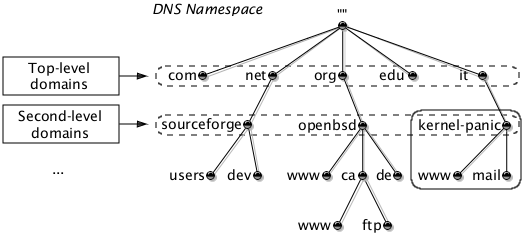
\includegraphics[height=5cm]{../../slides/dns/images/namespace.png}
\end{frame}}
\mode<all>{\begin{frame}
    \frametitle{Определения}
    \begin{block}{Домен domain}
    узел в дереве имён, вместе со всеми подчинёнными ему узлами, то есть именованная ветвь или поддерево в дереве имён.
    \end{block}
    \begin{block}{Поддомен subdomain}
         — подчинённый домен например, wikipedia.org — поддомен домена org, 
         ru.wikipedia.org — поддомен домена wikipedia.org
    \end{block}
    \begin{block}{Делегирование}
     передача ответственности за ветвь DNS другому лицу
    \end{block}
\end{frame}
}
\mode<all>{
\begin{frame}[fragile]
  \frametitle{Протокол DNS}
\begin{itemize}
  \item TCP или UDP
  \item \alert{порт 53} для ответов на запросы
  \item запросы и ответы отправляются в виде одной \alert{UDP}-датаграммы. 
  \item когда размер данных ответа > 512 байт используется \alert{TCP}
\end{itemize}

\end{frame}
}
\section{Client.}
\mode<all>{\begin{frame}
  \frametitle{Клиент}

\begin{block}{DNS-клиент} 
  специализированная библиотека (или программа) для работы с DNS.
\end{block} 

\begin{block}{Рекурсия}
  алгоритм поведения DNS-сервера: выполнение от имени клиента полный поиск нужной информации во всей системе DNS, при необходимости обращаясь к другим DNS-серверам.
\end{block}

\begin{block}{рекурсивным запрос} 
  требующим полного поиска
\end{block}

\begin{block}{нерекурсивным (или итеративным) запрос} 
  не требующим полного поиска.
\end{block}

\end{frame}}
\mode<all>{\begin{frame}[fragile]
  \frametitle{resolv.conf}
/etc/resolv.conf
\begin{lstlisting}
nameserver 192.168.1.101
nameserver 192.168.1.102
domain  unixmen.local
\end{lstlisting}

\end{frame}}
\mode<all>{\begin{frame}
  \frametitle{DNS клиент.}
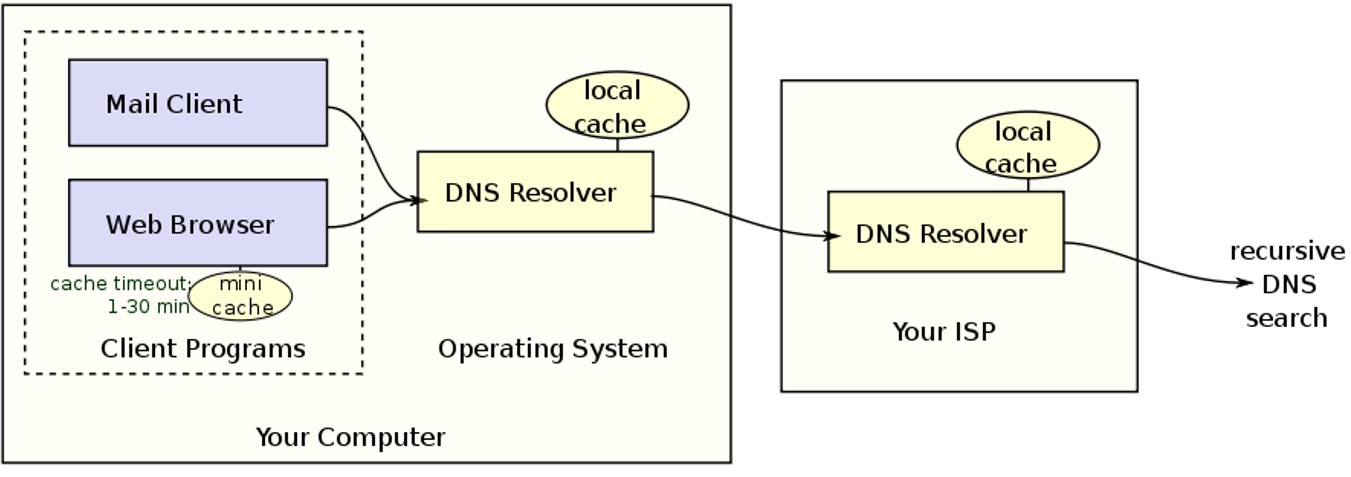
\includegraphics[height=4cm]{../../slides/dns/images/dns_resolver.png}
\end{frame}}
\mode<all>{\begin{frame}{fragile}
  \frametitle{Процесс получения ответа на запрос}
\begin{center}
  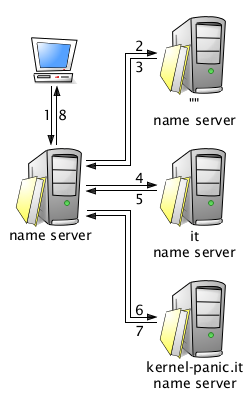
\includegraphics[height=5cm]{../../slides/dns/images/resolvprocess.png}
\end{center}
\end{frame}}
\mode<all>{\begin{frame}[fragile]
  \frametitle{Установка команд клиентов DNS}

CentOS
\begin{lstlisting}
yum install bind-utils
\end{lstlisting}

Ubuntu
\begin{lstlisting}
apt install bind9utils dnsutils
\end{lstlisting}
  
\begin{itemize}
  \item dig
  \item host
  \item nslookup
\end{itemize}

Посылают запросы напрямую к DNS серверу минуя резолвер операционной системы

\end{frame}
}
\mode<all>{\begin{frame}[fragile]
    \frametitle{Выполняем запросы}
Узнаем IP адрес
\begin{lstlisting}
host www.it-academy.by
dig www.it-academy.by
nslookup www.it-academy.by
\end{lstlisting}

Узнаем куда слать почту, адреса DNS серверов, текст и прочее. 

Как это сделать?
\begin{lstlisting}
    dig NS www.it-academy.by
    dig MX it-academy.by
    dig SOA www.it-academy.by
    dig TXT it-academy.by
\end{lstlisting}

\end{frame}}
\mode<all>{\begin{frame}[fragile]
    \frametitle{Выполняем полный поиск вручную}
Определим DNS сервера домена ya.ru
\begin{lstlisting}
dig 
dig   @d.root-servers.net ya.ru ns
dig   @b.dns.ripn.net. ya.ru ns
dig   @ns1.yandex.RU. ya.ru a

dig +trace cheat.sh
\end{lstlisting}
\end{frame}}
\section{Server Bind.}
\mode<all>{\begin{frame}
    \frametitle{Сервер}
   \begin{block}{DNS-сервер}
    специализированное ПО для обслуживания DNS, а также компьютер, на котором это ПО выполняется.
   \end{block} 
    \begin{block}{Зона}
     часть дерева доменных имен, размещаемая как единое целое на DNS-сервере 
    \end{block}
\end{frame}}
\mode<all>{\begin{frame}
    \frametitle{Реализации сервера}
    \begin{itemize}
        \item \alert{BIND} -  (Berkeley Internet Name Domain, ранее: Berkeley Internet Name Daemon)
        \item \alert{dnsmasq}
        \item \alert{PowerDNS}
        \item \alert{unbound}
    \end{itemize}

\end{frame}}
\mode<all>{\begin{frame}
    \frametitle{Роли сервера}

\begin{block} { Master-сервер (primary, первичный)}
     хранит настройки зон
\end{block}
\begin{block}{ Slave-сервер (secondary, вторичный, дублирующий)}
    копирует настройки с первичного
\end{block}
Вторичные сервера предоставляют избыточность и распределяют нагрузку
\begin{block}{Cache-сервер (кэширующие)}
нет описания зон, хранит кэш запросов
\end{block}
    

\end{frame}}
\mode<all>{\begin{frame}
    \frametitle{Ресурсные записи}
\begin{itemize}
    \item \alert{A} — (address record/запись адреса) отображают имя хоста (доменное имя) на адрес IPv4. 
    \item \alert{NS} (name server/сервер имён) указывает на DNS-сервер, обслуживающий данный домен. 
    \item \alert{SOA} (Start of Authority/начальная запись зоны) — описывает основные/начальные настройки зоны, можно сказать, определяет зону ответственности данного сервера. 
    \item \alert{SRV} используется в Active Directory
    \item \alert{TXT} текстовая информация
\end{itemize}


\end{frame}}
\section{SOA record.}
\mode<all>{\begin{frame}[fragile]
    \frametitle{Пример записи}
    
\begin{lstlisting}
unixmen.local   IN  SOA     masterdns.unixmen.local. root.unixmen.local. (
    2014071001  ;Serial (серийный номер)
    3600        ;Refresh (обновление)
    1800        ;Retry (повторная попытка)
    604800      ;Expire (срок годности)
    86400       ;Minimum TTL (минимальное время жизни)
\end{lstlisting}

\end{frame}}
\mode<all>{\begin{frame}[fragile]
    \frametitle{Значения SOA}

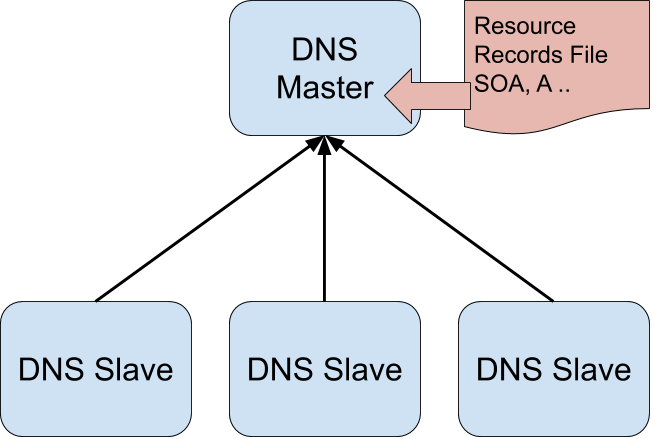
\includegraphics[height=5cm]{../../slides/dns/masterslave.png}

\end{frame}}
\mode<all>{\begin{frame}[fragile]
    \frametitle{Практика найти значения}

Выполнить команду
\begin{verbatim}
    dig xy.com SOA
\end{verbatim}
Найти AUTHORITY SECTION и в ней определить значения
\begin{itemize}
    \item Serial
    \item Refresh 
    \item Retry 
    \item Expire 
    \item Minimum TTL
\end{itemize}
Через время TTL выполнить команду и сравнить Query time:
\begin{verbatim}
dig xy.com
\end{verbatim}

\end{frame}}
\end{document}
